\documentclass{beamer}

\usetheme{Rochester}
\usecolortheme{material}
\usepackage{multicol}

\setbeamertemplate{footline}[text line]{%
  \parbox{0.5\linewidth}{
    \vspace*{-12pt} %\insertshorttitle~(\insertshortauthor)
  }
  \hfill%
  \parbox{0.5\linewidth}{
    \vspace*{-12pt}\raggedleft\insertpagenumber
  }
}
\setbeamertemplate{navigation symbols}{}
\begin{document}
\title[Entwurssprachen]{HW/SW Entwurfssprachen am Beispiel System-C}
\author[Zaruba F., Weber T.]{Florian Zaruba, Thomas Weber}
\date{\today} 

\begin{frame}
\titlepage
\end{frame}

\begin{frame}\frametitle{Table of contents}
%\begin{multicols}{2}
  \tableofcontents
%\end{multicols}
\end{frame}


\section{HW/SW Design Languages} 

\begin{frame}\frametitle{Motivation} 
tba
\begin{itemize}
	\item Rapidly increasing number of embedded systems.
	\item complexity (! graph)
\end{itemize}
\end{frame}

\begin{frame}\frametitle{System-Level Description Language (SDL)} 
\begin{itemize}
	\item Specification and design at various abstraction levels
	\item Faster design cycles %? 
\end{itemize}
\end{frame}

\section{SystemC Overview}
\begin{frame}\frametitle{What is SystemC}
\begin{itemize}
	\item Set of C++ classes and macros (Concurrency and notion of time)
	\item Common language for SW and HW, C++
	\item Enhanced productivity, higher abstraction level (TLM)
\end{itemize}
\end{frame}

\subsection{History}
\begin{frame}\frametitle{History} 
tba
\end{frame}


\begin{frame}\frametitle{Where does it fit in?} 
	    \begin{figure}[hp]
	      \centering
	      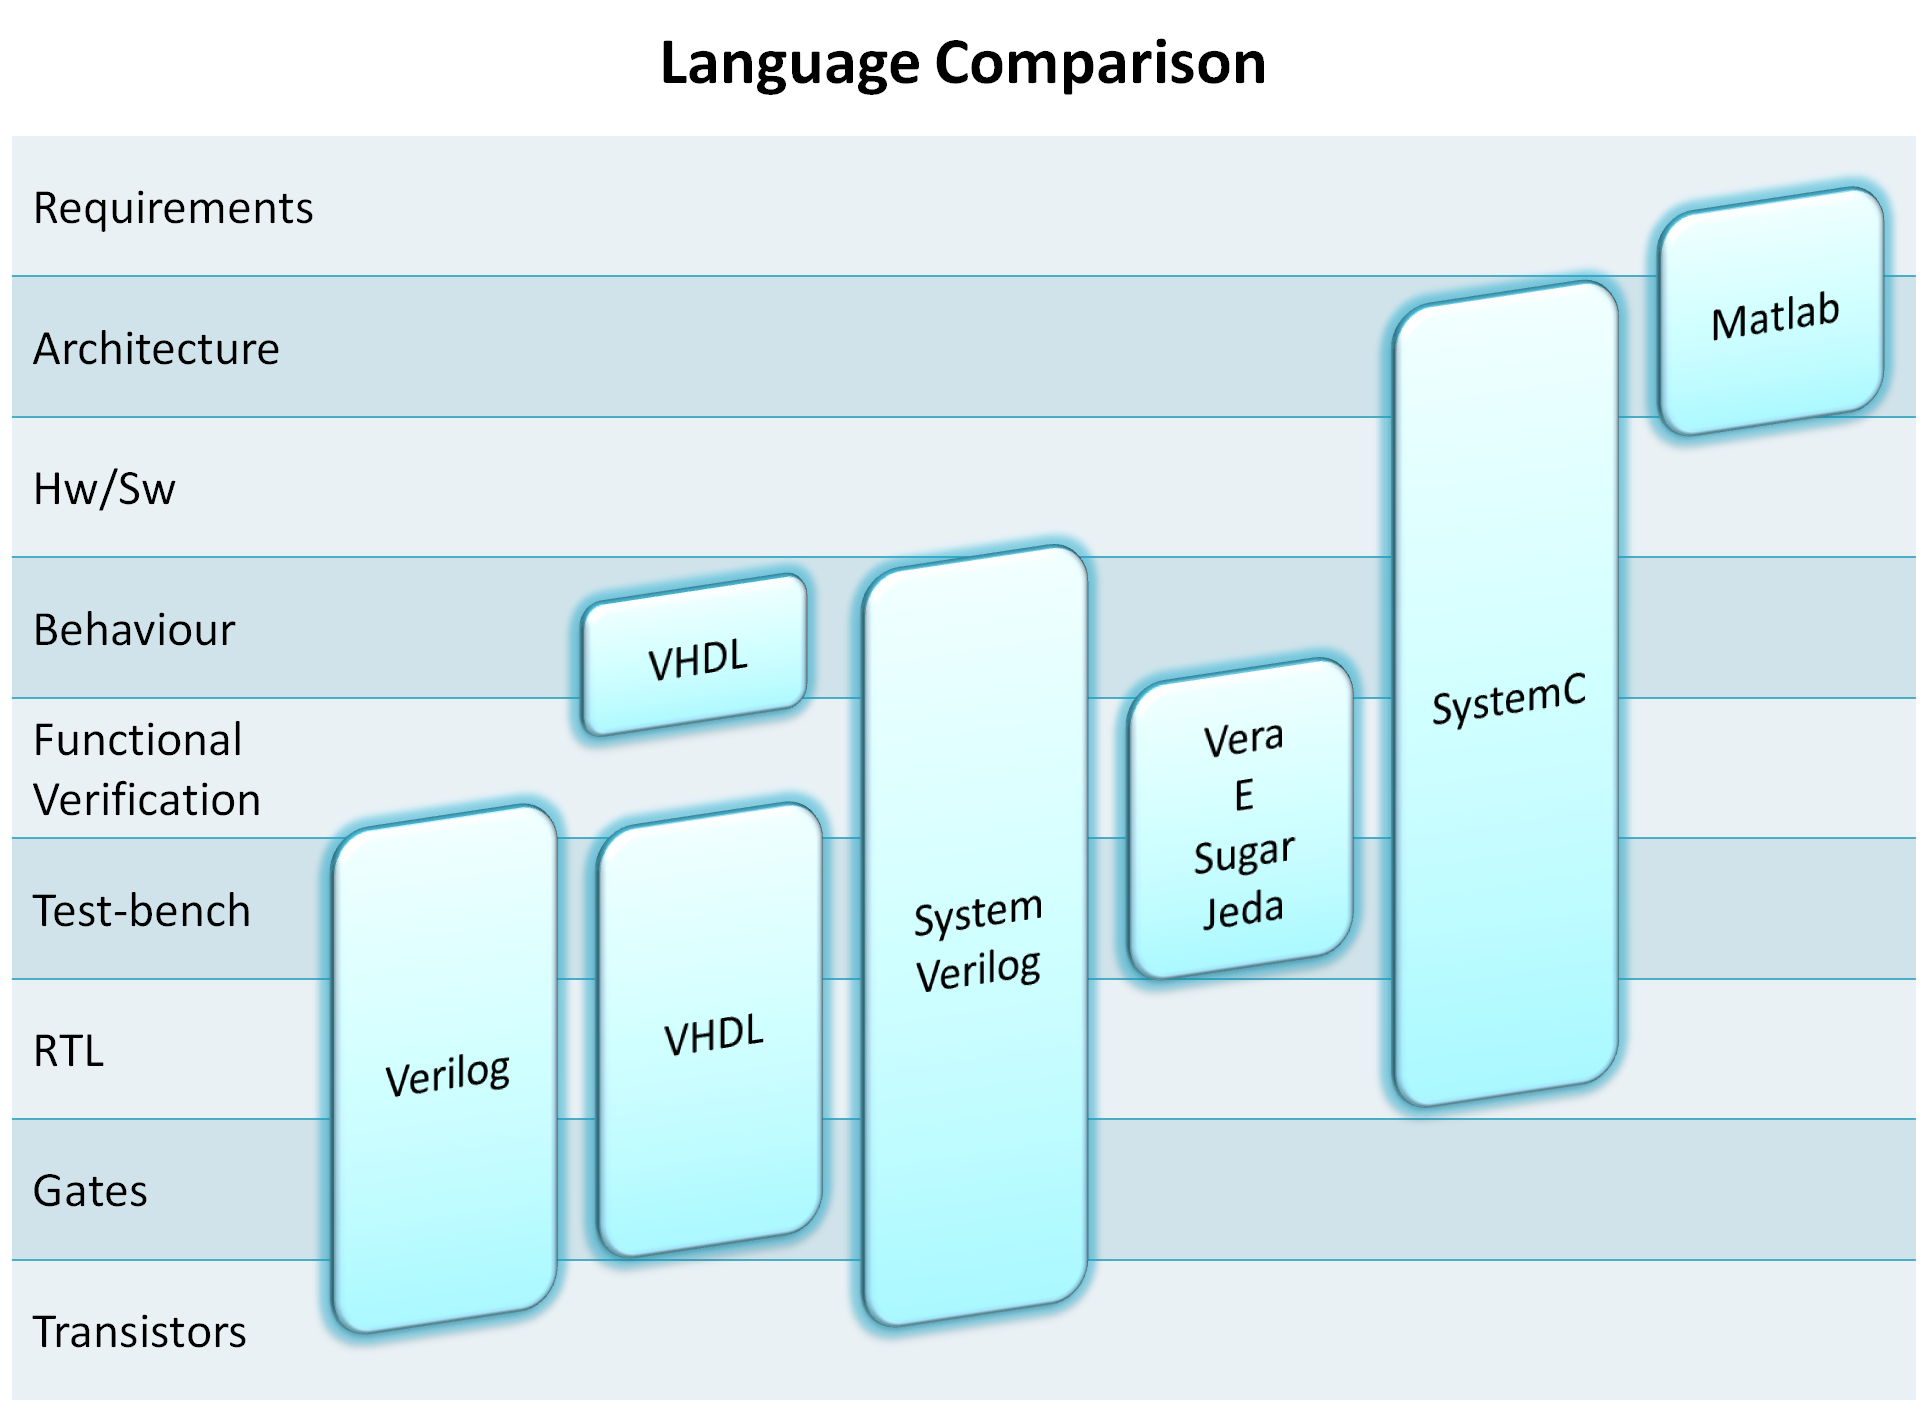
\includegraphics[width=0.7\textwidth]{pictures/Hardware_Description_Languages_and_Abstraction_Levels.png}
	      \caption{Hardware Description Languages and Abstraction Levels\footnote[frame]{\url{http://www.esa.int/Our_Activities/Space_Engineering/Microelectronics/System-Level_Modeling_in_SystemC}}}
	      \label{fig:flow}
	    \end{figure} 

\end{frame}

\subsection{Benefits/Drawbacks}
\begin{frame}\frametitle{Benefits} 
tba
\begin{itemize}
	\item Lot of C++ tools already available and useful
\end{itemize}
\end{frame}
\begin{frame}\frametitle{Drawbacks} 
tba
\end{frame}

\subsection{Differences to other languages}
\begin{frame}\frametitle{SysC vs. C} 
tba
\end{frame}
\begin{frame}\frametitle{SysC vs. VHDL} 
tba
\end{frame}

\subsection{Examples - Comparison}
\begin{frame}\frametitle{SysC vs. C} 
Code von Thomas
\end{frame}
\begin{frame}\frametitle{SysC vs. VHDL} 
Code von Thomas
\end{frame}


\section{Automatic Partitioning}
\begin{frame}\frametitle{Automatic Partitioning} 

\begin{block}{title of the bloc}
bloc text
\end{block}

\begin{exampleblock}{title of the bloc}
bloc text
\end{exampleblock}


\begin{alertblock}{title of the bloc}
bloc text
\end{alertblock}
\end{frame}

\section{Tools}
\begin{frame}\frametitle{Tools} 
\textbf{SystemC to VHDL}

http://calypto.com/en 	Catapult SL/LP

http://www.forteds.com	Cynthesizer 5 

\textbf{SystemC Simulation}

Modelsim
\end{frame}

\section{Who uses it?}
\begin{frame}\frametitle{Users} 
tba
\end{frame}
      
\section{Bibliography}
\begin{frame}\frametitle{Literature} 
Haubelt, Christian. Digitale Hardware/Software-Systeme. Springer-Verlag, 2010.

\end{frame}



\end{document}
